\subsection{Программная реализация RSA}

\subsubsection{Структура класса и зависимости}
Реализация инкапсулирована в класс `RSA`, который наследуется от абстрактного базового класса `Protocol`. Это позволяет в будущем легко интегрировать другие криптографические протоколы в единую систему. В заголовочном файле `rsa.hpp` определена структура класса и его основные компоненты.

\begin{nvimstyle}
#ifndef RSA_HPP
#define RSA_HPP

#include "protocol.hpp"

#include <boost/multiprecision/cpp_int.hpp>
#include <boost/random/mersenne_twister.hpp>

using BigInt = boost::multiprecision::cpp_int;

namespace CRYPTO
{
class RSA final : public Protocol
{
public:
	explicit RSA(unsigned int key_bits = 2048);

	void init() override;

	QString encrypt(const QString& plaintext) override;
	QString decrypt(const QString& ciphertext) override;

private:
	void generateKeys();
	BigInt generatePrime(unsigned int bits, boost::random::mt19937& rng);

	// Параметры RSA
	unsigned int m_key_bits;
	BigInt		 m_m; // Модуль m = p * q (часть открытого ключа)
	BigInt		 m_e; // Открытая экспонента e (часть открытого ключа)
	BigInt		 m_d; // Закрытая экспонента d (закрытый ключ)

	// Простые множители сохраняются для потенциального использования, но являются частью закрытого ключа
	BigInt m_p, m_q;
	BigInt m_phi; // Функция Эйлера: phi(n) = (p-1)*(q-1)
};
} // namespace CRYPTO

#endif // RSA_HPP

\end{nvimstyle}

\subsubsection{Генерация ключей}
Процесс генерации ключевой пары является наиболее важным и сложным этапом. Он реализован в методе `generateKeys()` и соответствует классическому алгоритму.

\begin{enumerate}
    \item \textbf{Генерация простых чисел $p$ и $q$.} Для этого используется вспомогательный метод `generatePrime()`, который генерирует случайное число заданной битовой длины и проверяет его на простоту с помощью вероятностного теста Миллера–Рабина. В реализации используется 25 итераций теста, что обеспечивает чрезвычайно высокую вероятность того, что сгенерированное число действительно является простым. Генерация продолжается до тех пор, пока не будут найдены два различных простых числа.
    
    \item \textbf{Вычисление модуля $m$ и функции Эйлера $\varphi(m)$.} Модуль вычисляется как $m = p \cdot q$, а значение функции Эйлера — как $\varphi(m) = (p-1)(q-1)$.
    
    \item \textbf{Выбор открытой экспоненты $e$.} В качестве открытой экспоненты выбрано стандартное значение $e = 65537$. Это число является простым и имеет всего два единичных бита в двоичном представлении ($2^{16}+1$), что позволяет значительно ускорить операцию возведения в степень при шифровании. Производится проверка, что $\text{НОД}(e, \varphi(m))=1$.
    
    \item \textbf{Вычисление секретной экспоненты $d$.} Секретная экспонента $d$ вычисляется как мультипликативное обратное к $e$ по модулю $\varphi(m)$, то есть $d \equiv e^{-1} \pmod{\varphi(m)}$. Для этого используется расширенный алгоритм Евклида, реализованный в отдельной функции `inverse()`.
\end{enumerate}


\begin{nvimstyle}
BigInt RSA::generatePrime(unsigned int bits, boost::random::mt19937& rng)
{
	// Задаем диапазон для генерации числа с нужным количеством бит
	BigInt											lower_bound = BigInt(1) << (bits - 1);
	BigInt											upper_bound = (BigInt(1) << bits) - 1;
	boost::random::uniform_int_distribution<BigInt> dist(lower_bound, upper_bound);

	BigInt candidate;
	while (true)
	{
		candidate = dist(rng);
		// Убедимся, что число нечетное
		if (candidate % 2 == 0)
		{
			candidate++;
		}
		// Проверяем на простоту с помощью теста Миллера-Рабина
		// 25 итераций дают очень высокую вероятность того, что число простое
		if (boost::multiprecision::miller_rabin_test(candidate, 25))
		{
			return candidate;
		}
	}
}
\end{nvimstyle}

\begin{nvimstyle}
void RSA::generateKeys()
{
    // 1. Инициализация генератора случайных чисел
    boost::random::mt19937 rng(std::chrono::high_resolution_clock::now().time_since_epoch().count());

    // 2. Генерация двух различных простых чисел p и q
    unsigned int prime_bits = m_key_bits / 2;
    do
    {
        m_p = generatePrime(prime_bits, rng);
        m_q = generatePrime(prime_bits, rng);
    } while (m_p == m_q);

    // 3. Вычисление модуля m и функции Эйлера phi(m)
    m_m   = m_p * m_q;
    m_phi = (m_p - 1) * (m_q - 1);

    // 4. Выбор открытой экспоненты e
    m_e = 65537;
    if (boost::multiprecision::gcd(m_e, m_phi) != 1)
    {
        // В маловероятном случае, если 65537 не подходит,
        // генерируем ключи заново
        generateKeys();
        return;
    }

    // 5. Вычисление закрытой экспоненты d
    m_d = inverse(m_e, m_phi);
}
\end{nvimstyle}

\subsubsection{Шифрование и расшифрование}
Процессы шифрования и расшифрования требуют преобразования текстовых данных в числовое представление и обратно.

\subsubsection*{Шифрование}
Метод `encrypt()` выполняет следующие шаги:
\begin{enumerate}
    \item Входная строка `QString` преобразуется в массив байтов `QByteArray` в кодировке UTF-8.
    \item Байтовый массив представляется в виде строки шестнадцатеричных символов. Это необходимо для однозначного преобразования двоичных данных в число.
    \item Шестнадцатеричная строка преобразуется в большое целое число `BigInt`.
    \item Производится проверка, что полученное число меньше модуля $m$.
    \item Выполняется основная операция шифрования: $c = s^e \pmod m$ с помощью функции `boost::multiprecision::powm`, оптимизированной для модульного возведения в степень.
    \item Полученный шифртекст $c$ преобразуется обратно в шестнадцатеричную строку для передачи.
\end{enumerate}

\begin{nvimstyle}
QString RSA::encrypt(const QString& plaintext)
{
    // 1. Преобразуем открытый текст в байты
    QByteArray bytes = plaintext.toUtf8();
    
    // 2. Преобразуем байты в шестнадцатеричную строку.
    QString hex_plaintext = bytes.toHex();
    
    // 3. Преобразуем шестнадцатеричную строку в BigInt.
    BigInt message("0x" + hex_plaintext.toStdString());

    // 4. Проверяем, что сообщение меньше модуля n
    if (message >= m_m)
    {
        throw std::runtime_error("Message is too large for the current key size.");
    }

    // 5. Шифруем: c = m^e mod n
    BigInt ciphertext = boost::multiprecision::powm(message, m_e, m_m);

    // 6. Преобразуем зашифрованное число в строку в шестнадцатеричном формате
    return QString::fromStdString(ciphertext.str(0, std::ios_base::hex));
}
\end{nvimstyle}

\subsubsection*{Расшифрование}
Метод `decrypt()` выполняет обратную последовательность действий:
\begin{enumerate}
    \item Входной шифртекст в виде шестнадцатеричной строки преобразуется в большое целое число `BigInt`.
    \item Выполняется операция расшифрования: $s = c^d \pmod m$ с помощью функции `powm`.
    \item Расшифрованное число преобразуется обратно в шестнадцатеричную строку.
    \item На этом этапе выполняется важная коррекция: если полученная строка имеет нечетную длину, в начало добавляется ведущий ноль. Это необходимо, так как при преобразовании числа в строку `0x0F` может превратиться в `"f"` вместо `"0f"`, что приведет к ошибке на следующем шаге.
    \item Скорректированная шестнадцатеричная строка преобразуется в `QByteArray`, а затем в `QString` в кодировке UTF-8, восстанавливая исходное сообщение.
\end{enumerate}

\begin{nvimstyle}
QString RSA::decrypt(const QString& ciphertext)
{
    // 1. Преобразуем шифротекст в BigInt
    BigInt encrypted_message("0x" + ciphertext.toStdString());

    // 2. Расшифровываем: m = c^d mod n
    BigInt decrypted_message = boost::multiprecision::powm(encrypted_message, m_d, m_m);

    // 3. Преобразуем расшифрованное число обратно в шестнадцатеричную строку
    std::string hex_str = decrypted_message.str(0, std::ios_base::hex);

    // 4. Восстанавливаем возможный утерянный ведущий ноль
    if (hex_str.length() % 2 != 0)
    {
        hex_str.insert(0, "0");
    }

    // 5. Преобразуем шестнадцатеричную строку обратно в QByteArray
    QByteArray bytes = QByteArray::fromHex(QByteArray::fromStdString(hex_str));

    // 6. Создаем QString из байтов в кодировке UTF-8
    return QString::fromUtf8(bytes);
}
\end{nvimstyle}

\subsection{Пример работы RSA}
\begin{figure}[htbp]
    \centering 
    \subfloat[Encryption]{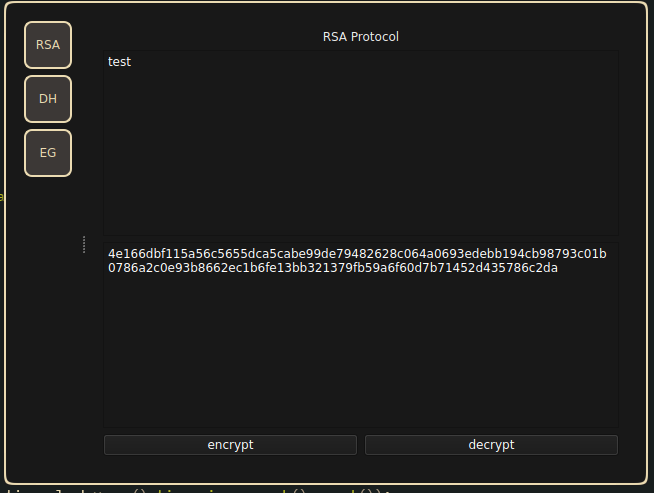
\includegraphics[width=0.48\textwidth]{res/png/00_rsa_encrypt.png}\label{fig:sub1}}
    \hfill
    \subfloat[Decryption]{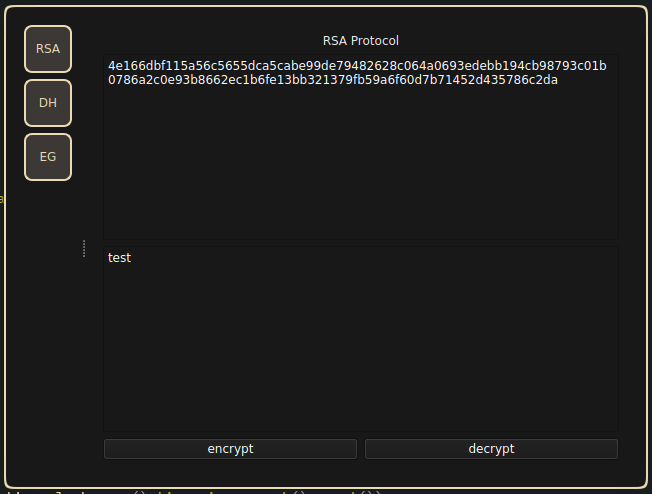
\includegraphics[width=0.48\textwidth]{res/png/01_rsa_decrypt.png}\label{fig:sub2}}
    \label{fig:side_by_side}
\end{figure}